\cotefile{157-3}
\scanpage{207}
\mspage{156}

du foncteur $\varphi_Q\colon\mathcal X\longrightarrow Y$, qu'on a \unsure{oublié} d'expliciter dans 3.2. Ça a vraiment l'air de marcher (comme sur des roulettes).

Appliquons le lemme 2 \deleted{\unsure{au}} au diagramme carré $Q_{/x_0}$ et à $\varphi_{(Q_{/x_0})}$ (page 154), on voit donc que les fibres à examiner \inserted{en les $\deleted{\unsure{x|u}}u\in\operatorname{Ob}Y_{/y}$ $(u\colon y'\longrightarrow y)$} peuvent s'écrire comme des intégrales

\diagram{\begin{tikzcd}[ampersand replacement=\&,row sep=small,column sep=small]
\& (X_{1/x_1})_u\\
\mathcal X(x_0,u)\overset{\text{déf}}{=}\displaystyle\int (X_{0/x_0})_u \arrow[ur]\arrow[dr] \&\\
\& (X_{2/x_2})_u .
\end{tikzcd}}

\deleted{\unsure{U}}Utilisons maintenant le fait que $f_1,f_2$ sont $W$-lisses (exprimant que $\varphi_Q$ est $W$-lisse dans $\mathcal X-X_0$), donc \deleted{que} \unsure{:} $(X_{1/x_1})_u$ et $(X_{2/x_2})_u$ sont $W$-asphériques. Dans le carré $W$-cocartésien

\diagram{\begin{tikzcd}[ampersand replacement=\&,row sep=small,column sep=small]
\& (X_{1/x_1})_u \arrow[dr,"{\unsure{f_1|i_1|j_1}(x_0,u)}",""{name=branchabove,near start}] \&\\
(X_{0/x_0})_u \arrow[ur,"{\alpha_1(x_0,u)}"]\arrow[dr,"{\alpha_2(x_0,u)}"'] \& \& (\mathcal X_{/x_0})_u \simeq \mathcal X(x_0,u) ,\\
\& (X_{2/x_2})_u \arrow[ur,"{i_2(x_0,u)}"',""{name=branchbelow,near start}]\arrow[from=branchabove,to=branchbelow,dashed,no head,shorten <=4pt,shorten >=4pt] \&
\end{tikzcd}}

% slanted
\margin{$\circ$ Attention \unsure{ce|on} n'est pas un carré commutatif. Dire plutôt que $(\mathcal X_{/x_0})_u\simeq\int$
\diagram{\begin{tikzcd}[ampersand replacement=\&,row sep=0pt,column sep=4pt]
\& {}\\[-3pt]
{} \arrow[ur]\arrow[dr] \&\\[-3pt]
\& {}
\end{tikzcd}}
est lisse sur $\underline{\Phi}$, à fibres $W$-asphériques (si $f_0,f_1,f_2$ sont lisses) donc $W$-as, \unsure{il faudrait que puisque} $\underline{\Phi}$ \unsure{l'est}.}

% slanted
\margin{\deleted{Au lieu de $W$\unsure{$(7')$} (bis) il suffit de \unsure{de plus|plus} supposer que \unsure{Cat muni du système} \unsure{est une 2-cat.} ? \unsure{$(\underline W,\underline{\Phi W})$} \unsure{cofinal triang.} ! \unsure{?} pour la \unsure{partie} \unsure{$f_1,f_2,f_0$ lisses} $\Rightarrow$ \unsure{$\varphi$ lisse}. C'est \unsure{moins fort} que cette \unsure{assertion}, car alors les \unsure{diff.} iso, sont \unsure{des} \illegible{1}.}}

``$(\mathcal X_{/x_0})_u$ est $W$-\unsure{asphérique|asph.}'' \unsure{et} $(X_{1/x_1})_u$ et $(X_{2/x_2})_u$ le \unsure{sont|sont-elles} \unsure{équivalent|équivalant} à $i_1(x_0,u)\in W$ (ou $i_2(x_0,u)\in W$) donc aussi \unsure{(moyennant $W(7\ \mathrm{bis})$)} :
% archive sheet number: 207
\scanpage{208}
\mspage{157}

\[
\alpha_1(x_0,u)\in W\quad\text{\unsure{i.e.}}\quad (X_{0/x_0})_u\quad W\text{-asphérique}.
\]

\deleted{Cela signifie} Dire que c'est vrai pour tt $u$ dans \deleted{\unsure{la}} $Y_{/y}$, signifie que $f_0\colon X_0\unsure{-|\longrightarrow}Y$ est lisse en \unsure{$x$|$x_0$|$u$}.

Donc on a prouvé a), sous la forme plus précise :

\uline{Corollaire 6} \deleted{\unsure{en supposant $W(7\ \mathrm{bis})$|On suppose $W(7\ \mathrm{bis})$}} Soit $x\in\operatorname{Ob}\mathcal X$ (où

\diagram{\begin{tikzcd}[ampersand replacement=\&,row sep=0pt,column sep=small]
\& X_1\\
\mathcal X=\displaystyle\int X_0 \arrow[ur,dash]\arrow[dr] \&\\
\& X_2
\end{tikzcd}}

). On veut exprimer la \inserted{$W$-}lissité de \deleted{\unsure{$\varphi$}}

\[
\varphi_Q\colon\mathcal X\unsure{-|\longrightarrow}Y
\]

en $x$.

a) Si $x\in\operatorname{Ob}X_i$ $(i\in\{1,2\})$, $\varphi_Q$ est \inserted{$W$-}lisse en $x$ ssi $f_i\colon X_i\unsure{-|\longrightarrow}Y$ l'est.

b) Supposons $W(7\ \mathrm{bis})$\textsuperscript{*}. \deleted{Si $x\in\operatorname{Ob}X_0$,} \inserted{Soit $x_0\in\operatorname{Ob}X_0$, et supposons $f_1,f_2$ lisses en $x_1,x_2$.} Alors $\varphi_Q$ est $W$-lisse en \unsure{$x_0$} ssi $f_0\colon X_0\longrightarrow Y$ l'est.

% slanted
\margin{Inutile pour la partie directe, en supposant}

Donc \inserted{(moyennant $W(7\ \mathrm{bis})$)} dans \deleted{les} les trois cas $x\in\operatorname{Ob}X_i$ $(i\in\{0,1,2\})$, on trouve que $\varphi_Q$ est \inserted{$W$-}lisse en $x$ ssi $f_i\colon X_i\unsure{-|\longrightarrow}Y$ l'est.

Quant à b) du \deleted{\unsure{la prop. II|le princ. II|la prop. 15}}, \inserted{th. \deleted{\illegible{1}}} c'est le lemme 2 ci-dessus. Donc tout est prouvé !
% archive sheet number: 208
\scanpage{209}
\mspage{158}

\uline{3.5}. \uline{\unsure{Application|Applications} aux sommes amalgamées dans une catégorie} $X^\wedge$ (avec $X\in\operatorname{Ob}\mathrm{Cat}$).

D'abord une caractérisation des sommes amalgamées impliquant une imm. ouverte :

\uline{Proposition 15} Soit

\diagram{\begin{tikzcd}[ampersand replacement=\&]
\& U \arrow[r,hook,"i"]\arrow[d,"{\unsure{r|p}}"'] \& X\arrow[d,"q"]\\
Q\colon \& U' \arrow[r,"i'"] \& X'
\end{tikzcd}}

un carré commutatif dans Cat. Pour que ce carré soit cocartésien\inserted{ dans Cat}, avec $i$ (donc $i'$) une imm. ouverte, il faut et il suffit que les conditions suivantes soient satisfaites :

\inserted{a) $Q$ est cartésien,}

\deleted{\unsure{a}}b) $i'$ est une immersion ouverte (donc $i$ aussi),

\deleted{b) $Q$ est cartésien}

c) Si $T'=X'\setminus U'$, et $T=X\times_{X'}T'\inserted{=X\setminus U}$, $T\longrightarrow T'$ est un iso.

d) Pour tout $t\in T$, si $t'$ est son image dans $T'$, le foncteur induit par $p$

\[
p_{/t}\colon
\underset{\substack{\shortparallel\\ V_t}}{U_{/t}}
\longrightarrow
\underset{\substack{\shortparallel\\ V'_{t'}}}{U'_{/t'}}
\]

\deleted{\unsure{satis}} \deleted{\unsure{est à}} satisfait : $(p_{/t})_!(e_{U/t})\simeq e_{U'/t'}$, ou ce qui revient au $=$, les ``fibres colocales'' de $p_{/t}$, $v'\backslash V_t$ avec $v'$ dans $V'_{t'}$, sont $0$-connexes.
% archive sheet number: 209
\scanpage{210}
\mspage{159}

Démonstration immédiate - \unsure{ça|Ça} devrait plutôt remonter au § 1.

\uline{Corollaire 1} Soit $Q$ un carré \uline{cartésien} (cf page 158) avec $i'$ une \uline{imm. ouverte} (donc $i$ aussi), et $q$ \inserted{$W$-}\uline{lisse} (donc $p$ aussi). On suppose que $W$ satisfait l'axiome $W(5)$ de connexité. Soit $T'=X'\setminus U'$, $T=X\setminus U$, supposons que $T'\unsure{-|\longrightarrow}T$ soit un isomorphisme. Alors $Q$ est cocartésien.

% slanted
\margin{Donc il suffit $q$ $W_0$-lisse, où $W_0=\{f\in\operatorname{Fl}\mathrm{Cat}\mid\unsure{\pi_0|\Pi_0}(f)\text{ bijectif}\}$}

Il suffit de prouver la condition d)\inserted{ de prop. 15}. Considérons le carré

\diagram{\begin{tikzcd}[ampersand replacement=\&]
\& U_{/t}\arrow[r,hook,"i_{/t}"]\arrow[d,"p_{/t}"'] \& X_{/t}\arrow[d,"q_{/t}"]\\
(\unsure{\alpha|a|*})\& U'_{/t'} \arrow[r,hook,"i'_{/t'}"] \& X'_{/t'} ,
\end{tikzcd}}

je dis qu'il est \uline{cartésien}. Cela résulte de \deleted{la} seule hypothèse que $Q$ soit cartésien, sans hyp. de lissité sur $q$ ni que $i'$ soit une imm. ouverte, et se voit p. ex. en regardant le \deleted{cube} diagramme cubique :

\diagram{\begin{tikzcd}[ampersand replacement=\&,row sep=small,column sep=small]
\& U_{/t}\arrow[rr]\arrow[dl]\arrow[dd,crossing over] \& \& X_{/t}\arrow[dl]\arrow[dd]\\
U'_{/t'}\arrow[rr,crossing over]\arrow[dd] \& \& X'_{/t'}\arrow[dd]\arrow[dl,phantom,"\deleted{\unsure{\swarrow}}" description] \&\\
\& U\arrow[dl]\arrow[rr,dash,crossing over] \&\& \unsure{X'|X}\arrow[dl]\\
U'\arrow[rr,dash] \& \& X'\arrow[ul,phantom,"\deleted{\unsure{\swarrow}}" description] \&
\end{tikzcd}}

\margin{NB ici $t$ est un élément quelc. de $\operatorname{Ob}X$, $t'$ son image dans $X'$}

Dans ce diagramme, les faces \unsure{antérieures} et \unsure{postérieures} du cube \unsure{est|sont} \unsure{cartésien|cartésiens|cartésiennes}, par définition de $U_{/t}$ et \deleted{\unsure{de}} $U'_{/t'}$
% archive sheet number: 210
\scanpage{211}
\mspage{160}

respectivement, et la base l'est par hypothèse. Il en résulte que la face supérieure du cube est également un carré cartésien.

Ceci vu, \deleted{\unsure{com}} \unsure{comme} $q$ est lisse, il en est de $=$ de $q_{/t}$ dans le carré cartésien $(\unsure{\alpha|a|*})$, donc aussi de $p_{/t}$ par changement de base. D'autre part, la lissité de $q$ implique que $q_{/t}$ est à fibres $W$-asphériques, donc par changement de base il en est de $=$ de $p_{/t}$ (qui est donc une $W$-équivalence universelle, i.e. une $W$-fibration triviale). De plus, \inserted{à cause de la lissité de $p_{/t}$,} pour $v'$ dans $U'_{/t'}$, l'inclusion

\[
(U_{/t})_{v'}\longrightarrow v'\backslash(U^{\deleted{\unsure{\prime}}}_{/t\deleted{\unsure{\prime}}})
\]

est dans $W$, donc (par $W(5)$) définit une bijection sur les $\unsure{\pi_0|\Pi_0}$. Comme $(U_{/t})_{v'}$ est $W$-asphérique par ce qui précède, il s'ensuit \inserted{(par $W(5)$)} que son $\pi_0$ est de cardinal 1, donc il en est de $=$ de $\unsure{v'(U_{/t})|v'\backslash(U_{/t})}$, i.e. celui-ci est $0$-connexe. Or c'est là la condition d) de la prop. \unsure{15|10} qu'il fallait établir.
% archive sheet number: 211
\scanpage{212}
\mspage{161}

\uline{Corollaire 2} Soit $Q$ un carré cartésien (p. 158), avec $i'$ (donc \inserted{aussi} $i$) une imm. ouverte, et $q$ \inserted{(donc aussi $p$)} un \uline{isom.} \uline{local}. \deleted{Supposons que \unsure{$T$}} \inserted{Soit $T=X\setminus U$, $T'=X'\setminus U'$} (donc $T\simeq X\times_{X'}T'$), et supposons $T'\longrightarrow T$ iso. Alors $Q$ est cocartésien.

C'est un cas particulier du cor. 1, mais sans référence explicite à un localiseur $W$. On peut prendre $W=W_\infty$, ou $W=W_0$, pour se ramener au corollaire 1. Mais il est plus raisonnable de dire que dans le carré cartésien $(*)$, l'hypothèse que $q$ soit un iso. local implique que $q_{/t}$ \unsure{est} un isomorphisme, donc $p_{/t}$ l'est aussi. Il en résulte bien que les $v'\backslash(U_{/t})$ sont $0$-connexes, \deleted{\unsure{si ce}} \deleted{\unsure{puis}} \unsure{cette|ces} \unsure{catégorie|catégories} \unsure{étant} isom. à $\unsure{v'(U'_{/t'})|v'\backslash(U'_{/t'})}$, donc a un objet initial.

\deleted{Consid} Soit maintenant $X$ un objet de Cat, et considérons un diagramme cocartésien dans $X^\wedge$ :

\diagram{\begin{tikzcd}[ampersand replacement=\&]
\& \unsure{G|G'}\arrow[r,hook,"i"]\arrow[d,"p"'] \& \unsure{F|F'}\arrow[d,"q"]\\
(\unsure{*|**})\& G'\arrow[r,hook,"i'"] \& F',
\end{tikzcd}}
% archive sheet number: 212
\scanpage{213}
\mspage{162}

où $i$ est un monomorphisme. On sait que le caractère cocartésien du carré se vérifie ``argument par argument'' par le caractère cocartésien de

\diagram{\begin{tikzcd}[ampersand replacement=\&]
\deleted{\unsure{F}}G(x)\arrow[r,hook,no head,"i(x)"]\arrow[d,"p(x)"'] \& F(x)\arrow[d,"q(x)"]\\
G'(x)\arrow[r,hook,no head,"i'(x)"] \& F'(x)
\end{tikzcd}}

dans Ens, $\forall x$ dans $X$. Or un \inserted{tel} carré cocartésien \unsure{sur|dans} $\unsure{\overline{\mathrm E}|\mathrm E}\mathrm{ns}$, avec $i(x)$ mono, est aussi cartésien. Cela implique que le carré $Q$ dans $X^\wedge$ est également cartésien.

Considérons \inserted{d'autre part} le foncteur canonique

\[
\varphi_X\colon F\longmapsto X/F\colon X^\wedge\longrightarrow\mathrm{Cat}
\]

Il vaut mieux, d'ailleurs, le regarder comme un foncteur

\[
\varphi_{\unsure{X|x}}\colon X^\wedge\longrightarrow\mathrm{Cat}_{/X},
\]

et je rappelle, pour mémoire, que ce foncteur est pleinement fidèle, et que son image essentielle est formée des catégories $X'$ sur $X$ telles que

\[
\unsure{\alpha'|X'}\mathrel{\unsure{-|\longrightarrow}}X
\]
% archive sheet number: 213
\scanpage{214}
\mspage{163}

soit un isom. local, ou ce qui revient au $=$, que \deleted{\unsure{ce soit un}} $X'$ soit \uline{\unsure{fibrée|fibré}} sur $X$ à fibres discrètes :

\[
\varphi_X\colon \unsure{X|{}'X}^\wedge
\overset{\approx}{\mathrel{\unsure{-|\longrightarrow}}}
\underbrace{\underline{\unsure{\mathrm{Faib}|\mathrm{Fib}}\mathrm{.disc.}}\,X}_{\substack{\text{catégories fibrées}\\\text{à fibres discrètes}}} ,
\]

Notons que toute flèche $X'\unsure{-|\longrightarrow}X''$ dans $\underline{\mathrm{Fib}}\,\underline{\mathrm{disc}}\,X$ \deleted{\unsure{qui}} est un isom. local (tautologique sur

\diagram{\begin{tikzcd}[ampersand replacement=\&,row sep=small,column sep=small]
X'_{/x'}\arrow[rr,dash]\arrow[dr,dash,"\mathrm{iso}"'] \& \& X''_{/x''}\arrow[dl,dash,"\mathrm{iso}"]\\
\& X_{/x} \&
\end{tikzcd}}

), ce qui montre que si on a un diagramme

\diagram{\begin{tikzcd}[ampersand replacement=\&,row sep=small,column sep=small]
X_1\arrow[dr]\& \& X_2\arrow[dl]\\
\& X_0\&
\end{tikzcd}}

dans $\underline{\mathrm{Fib}}.\underline{\mathrm{disc}}.\,X$, son produit fibré $X_3=\unsure{\alpha_1|X_1}\times_{X_0}X_2$ dans Cat est tel que $X_3\unsure{-|\longrightarrow}X_2$, est un iso. local, donc aussi $X_3\longrightarrow X$. C'est-à-dire $\underline{\mathrm{Fib.disc}}\,X$ est stable par produits fibrés. Ceci implique que les \deleted{foncteur $\varphi_X$ transforme produits fib} \inserted{produits fibrés existent dans} $\underline{\mathrm{Fib\,disc}}\,X$, et que ce sont les produits fibrés dans Cat, ou dans $\mathrm{Cat}_{/\unsure{x|X}}$.
% archive sheet number: 214
\scanpage{215}
\mspage{164}

De $=$ pour les produits \deleted{\unsure{dans}} finis dans \deleted{\unsure{$G$|$\mathcal C$}} $\underline{\mathrm{Fib\,disc}}\,X$, ce sont les produits finis dans $\mathrm{Cat}_{/\unsure{X|x}}$. Bref

\uline{Lemme 1} \unsure{Les|La} \deleted{$\underset{\leftarrow}{\mathrm{lim}}$ finies existent dans} \inserted{sous-catégorie pleine} $\underline{\mathrm{Fib\,disc}}\,X$ de $\mathrm{Cat}_{/X}$ est stable par $\underset{\leftarrow}{\mathrm{lim}}$ finies, donc les \deleted{foncteur d'inclusion} \inserted{\unsure{$\underset{\leftarrow}{\mathrm{lim}}$|finies} existent dans} $\underline{\mathrm{Fib\,disc}}\,X$ \deleted{\unsure{$F$}} et le foncteur d'inclusion

\[
\underline{\mathrm{Fib\,disc}}\,X\mathrel{\unsure{-|\longrightarrow}}\mathrm{Cat}_{/X}
\]

y commute, et en particulier transforme carrés cartésiens de $\underline{\mathrm{Fib\,disc}}\,X$ en carrés cartésiens de $\mathrm{Cat}_{/X}$, ou ce qui revient au $=$, de Cat. De plus, en vertu de l'équivalence

\[
\varphi_X\colon X^\wedge\xrightarrow{\approx}\underline{\mathrm{Fib\,disc}}\,X,\ \unsure{\subset|-}\,\mathrm{Cat}_{/X}
\]

le foncteur $\varphi_X$ de $X^\wedge$ dans $\mathrm{Cat}_{/X}$ est exact à gauche, \deleted{\unsure{dans}} particulier il transforme carrés cartésiens de $X^\wedge$ en carrés cartésiens de $\mathrm{Cat}_{/X}$, \unsure{ou} même de Cat.
% archive sheet number: 215
\scanpage{216}
\mspage{165}

Notons aussi qu'étant exact à gauche, le foncteur $\varphi_X$ de $X^\wedge$ dans $\mathrm{Cat}_{/\unsure{X|x}}$ transforme mono en mono. D'autre part :

\uline{Lemme 2} Les monomorphismes qui sont des isom. \deleted{\unsure{ouverts|ouvertes}} locaux sont exactement les imm. ouvertes. Donc \deleted{les} dans $\underline{\mathrm{Fib\,disc}}\,X$, les monomorphismes sont les immersions ouvertes, et le foncteur $\varphi_X\colon F\longmapsto X/F$ transforme un monomorphisme en \unsure{immersion ouverte|immersions ouvertes}.

Revenons alors au diagramme cocartésien $(\unsure{*|\alpha})$ (p. 161), et au diagramme correspondant dans Cat (et $=$ dans $\underline{\mathrm{Fib\,disc}}\,X$)

\diagram{\begin{tikzcd}[ampersand replacement=\&]
X/G\arrow[r,hook,"X/i"]\arrow[d,"X/p"']\& X/F\arrow[d,"X/q"] \& T\unsure{{:}|\prime|{}}\arrow[l,dotted,hook]\arrow[d,dotted]\\
X/\unsure{G'|G''}\arrow[r,hook,"X/i'"]\& X/F' \& T'\arrow[l,dotted,hook] .
\end{tikzcd}}

Comme $(*)$ est cartésien, le carré précédent est cartésien, par ce qui précède. Je veux prouver qu'il est également cocartésien\unsure{,|.}
% archive sheet number: 216
\scanpage{217}
\mspage{166}

(dans $\mathrm{Cat}_{/\unsure{X|x}}$, ou dans Cat, cela revient au $=$), et pour ceci j'applique le cor. 2 de la prop. 15 (p. 161), compte tenu que $X/q$ est un iso. local, et $X/i'$ (étant un iso. local mono) une immersion ouverte. Il suffit de prouver que, \deleted{\unsure{dans}} $T'$ et $T$ étant les \deleted{\unsure{fermés}} sous-catégories fermées complémentaires des ouverts $X/G'$ de $X/F'$ et $X/G$ de $X/F$, que $T\unsure{-|\longrightarrow}T'$ est iso.

La vérification est immédiate \unsure{;} $T$ est la cat. des \inserted{flèches} $x\longrightarrow G$ \deleted{qui} \inserted{dans $X^\wedge$} \inserted{(de source $x$ dans $X$)} qui ne se factorisent pas par $G$, $T'$ celle des flèches $x\longrightarrow G'$ qui ne se factorisent pas par $F'$,

\diagram{\begin{tikzcd}[ampersand replacement=\&,row sep=small,column sep=small]
F\arrow[r,hook,no head]\arrow[d] \& G\arrow[d]\\
F'\arrow[r,hook,no head]\& G'
\end{tikzcd}}

le foncteur $T\mathrel{\unsure{-|\longrightarrow}}T'$ étant le foncteur composition de $x\longrightarrow G$ avec $G\xrightarrow{q}G'$.

\deleted{\unsure{Or}} (NB le composé ne se factorise pas par $F'$, car autrement, à cause du caractère cartésien de $Q$, $x\longrightarrow G$ se factoriserait par $F$). Mais pour $x$ donné, la donnée de $\deleted{G(x)}$ $x\longrightarrow G$ ne se factorisant pas par $F$ est celle d'un élément $\deleted{\unsure{G|\in}}$
% archive sheet number: 217
\scanpage{218}
\mspage{167}

de $G(x)\setminus F(x)$, et à cause du caractère cocartésien de $Q$,

\[
(G(x)\mathrel{\unsure{-|\setminus}}F(x))\mathrel{\unsure{-|\longrightarrow}}(G'(x)\unsure{>|\setminus}F'(x))
\]

est bijectif, i.e. ``il revient au $=$'' de se donner $x\mathrel{\unsure{-|\longrightarrow}}G$ ne se factorisant pas par $F$, ou $\unsure{a|x}\longrightarrow G'$ ne se factorisant pas par $F'$.

Ainsi on a prouvé le

\uline{Théorème 5} : Soit $X$ dans Cat, et

\diagram{\begin{tikzcd}[ampersand replacement=\&]
Q\colon \& F\arrow[r,hook,no head,"i"]\arrow[d,"\unsure{p|r}"']\& G\arrow[d,"q"]\\
\& F'\arrow[r,"i'"]\& G'
\end{tikzcd}}

un carré cocartésien dans $X^\wedge$, avec $i$ mono. Alors $i'$ est mono, le carré \inserted{$Q$} est aussi cartésien, et le carré correspondant dans $\mathrm{Cat}_{/X}$ ou dans Cat

\diagram{\begin{tikzcd}[ampersand replacement=\&]
X/F\arrow[r,"X/i"]\arrow[d,"X/p"'] \& X/G\arrow[d,dash,"X/q"]\\
X/\unsure{p'|P'|F'}\arrow[r,"X/i'"] \& X/G'
\end{tikzcd}}
% archive sheet number: 218
\scanpage{219}
\mspage{168}

est à la fois cartésien et cocartésien. De plus, si $W$ est un localiseur fondamental \unsure{dans|de} Cat, satisfaisant \deleted{\unsure{à}} $W(7\ \mathrm{bis})$ (en plus de $W(1,2,\unsure{3|13|{}'3})$), alors le \deleted{diagramme} carré $X/Q$ dans Cat est $W$-cocartésien.

Ce dernier énoncé résulte de ce qui précède et du cor. 2 du th. 4, compte tenu que $X/q$ est un iso. local donc est $W$-lisse.

\uline{Corollaire} : On a \inserted{(moyennant $W(7\ \mathrm{bis})$)} les équivalences

\[
\begin{aligned}
i\in W_X &\Longleftrightarrow i'\in W_X\\
p\in W_X &\Longleftrightarrow q\in W_X ,
\end{aligned}
\]

% slanted
\margin{\uline{NB} \unsure{Si on veut} seulement $i\in W_X\Rightarrow i'\in W_X$ $p\in W_X\Rightarrow q\in W_X$, il suffit que l'on ait $W(7\ \mathrm{bis})$ \uline{faible} i.e. $i_0\mathrel{\unsure{\in|\leftarrow}}W\Rightarrow i\in W$ dans l'énoncé de $W(7\ \mathrm{bis})$ \unsure{p. 76|p. 75} (Loc$(6'\mathrm a)$ avec les notations de $\underline{\overline{\mathrm{XVI}}}$)}

\[
W_X\subset\operatorname{Fl}(X^\wedge)
\]

est \unsure{défini|définie} par (cf. P. S. \ldots\ )

\[
\begin{aligned}
u\in W_X &\Longleftrightarrow X/u\colon X/F\unsure{-|\longrightarrow}X/G\\
&\hspace{4em}\text{est dans }W.
\end{aligned}
\]

Ainsi, dans une catégorie $X^\wedge$, les sommes amalgamées impliquant un mono se comportent de façon parfaite \unsure{du|au} point de vue homotopique, plus exactement pour les localiseurs $W_X$, pourvu
% archive sheet number: 219
\scanpage{220}
\mspage{169}

seulement que $W$ satisfasse \unsure{à|:} $W(7\ \mathrm{bis})$. Notamment, les monomorphismes dans $X^\wedge$ sont des ``$W_X$-cofibrations'', au sens \deleted{\unsure{si|de}} \unsure{similaire} de celui de la définition 2 c) (pages 99,100).

% paper watermark, sideways; last letter cut by the upper edge
\textsc{Strong} \unsure{\textsc{Extra}|\textsc{Extr}} \textsc{S}
% archive sheet number: 220
\scanpage{221}
\mspage{171}

\deleted{Dear Justine}
% typed cancellation: xxxxxxxxxxxx

$\overline{\underline{\mathrm{VI}}}$ \deleted{\uline{\unsure{Localiseurs|Localisation}} \unsure{de} \illegible{1} (\unsure{suite})}. \uline{Critère de} $W_\infty$-\uline{asphéricité par les} $\Omega^{\unsure{-|\bullet}}(X,\unsure{-|*})$.

\uline{1} \unsure{les conditions|les localiseurs|la filtration} \unsure{en|sur} $W_n$.

On va définir, pour $n\in\mathbb N$,

\[
 W_n\subset\operatorname{Fl}(\mathrm{Cat})\unsure{,|{;}}
\]

par les conditions suivantes (où $f:X\to Y$ est une flèche dans $\underline{\overline{\mathrm{Cat}}}$)

\[
 f\in W_0\iff\text{a) }\unsure{\pi_0|\Pi_0}(f)\ \text{bijectif}
\]

 \deleted{\unsure{$\Longleftrightarrow$ b)} le foncteur $F\mapsto f^*F$ des}
   
$\Longleftrightarrow$ \deleted{\unsure{b)}}c) le foncteur $F\mapsto f^*F$ des \inserted{\unsure{pré}}faisceaux d'ensembles \uline{constants} sur $Y$ vers les faisceaux d'ens. constants sur $X$ est pleinement fidèle

\margin{\figure{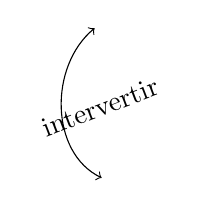
\begin{tikzpicture}
\draw[<->] (0.1,1) .. controls (-0.48,0.52) and (-0.47,-0.58) .. (0.19,-0.9);
\node[rotate=21] at (0.17,0) {\unsure{intervertir}};
\end{tikzpicture}}}
% slanted

$\Longleftrightarrow$ b) Pour tout préfaisceau d'ens. $F$ \uline{constant} sur $Y$,

\[
 H^0(Y,F)\longrightarrow \unsure{H^0|\mathcal H^0}(X,f^*F)\quad\text{est bijectif}
\]

\uline{NB} Si $F_0$ est un ensemble, $F_{0Y}$ le faisceau d'ens. constant défini par $F_0$ sur $Y$, on a

\[
\begin{aligned}
 H^0(Y,F_{0Y})&\simeq\operatorname{Hom}_{\mathrm{ens}}(\pi_0(Y),F_0)
    &&(\text{fonctoriel en }Y)\\
 \operatorname{Hom}_{Y^\wedge}(F_{0Y},G_{0Y})&\simeq
 \operatorname{Hom}_{\mathrm{ens}}(\pi_0(Y),\operatorname{Hom}_{\mathrm{ens}}(F_0,G_0))
    &&(\unsure{\text{id}^{\circ}|\text{id}})
\end{aligned}
\]

ce qui implique que

\[
 a\Longrightarrow \deleted{\unsure{b}}c
\underset{\substack{\text{en prenant}\\\operatorname{Hom}_{Y^\wedge}(e_Y,F)}}{\overset{\text{tautol}}{\Longrightarrow}}
\deleted{\unsure{c}}b\Longrightarrow a.
\]

$f\in W_1\Longleftrightarrow$ a) $\pi_0(f)$ bijectif, et pour tout $x\in\operatorname{Ob}X$,

\[
 \pi_1(f,x):\pi_1(X,x)\mathrel{\unsure{-|\to}}\pi_1(Y,f(x))\quad\text{est bijectif}
\]

(NB Il suffit de le vérifier pour \uline{un} $x$ dans chaque composante connexe de $X$.)

\[
 \text{a') }\Pi(X)\xrightarrow{\Pi f}\Pi(Y)\quad\text{est une équiv. de Cat.}
\]

$\Longleftrightarrow$ b) $H^0(\unsure{Y|X},F)\mathrel{\unsure{-|\to}}H^0(X,f^*(F))$ bijectif pour tout faisceau d'ens. \uline{loc.} \uline{constant} sur $Y$, et $H^1(Y,\deleted{\unsure{G}}F)\to H^1(Y,f^*F)$ bijectif \deleted{pour} \unsure{si} de plus $F$ est un faisceau en groupes.

\inserted{\unsure{b')|bis)} Comme b), mais pour le $H^1$ on se borne à $F$ \uline{constant}, et on exige $H^1(f)$ \uline{surjectif} \unsure{seulemt|seulement}.}

$\Longleftrightarrow$ c) Le foncteur $F\mapsto f^*F$ de la cat. des faisceaux d'ens. loc. constants sur $Y$ vers celle des faisceaux loc. const. sur $X$ est une équiv. de catégories.
% archive sheet number: 221
